\begin{figure}[!htbp]
    \centering
    \subfigure[CIU, tests on isotropically consolidated samples]{
        \label{figure:5a}
        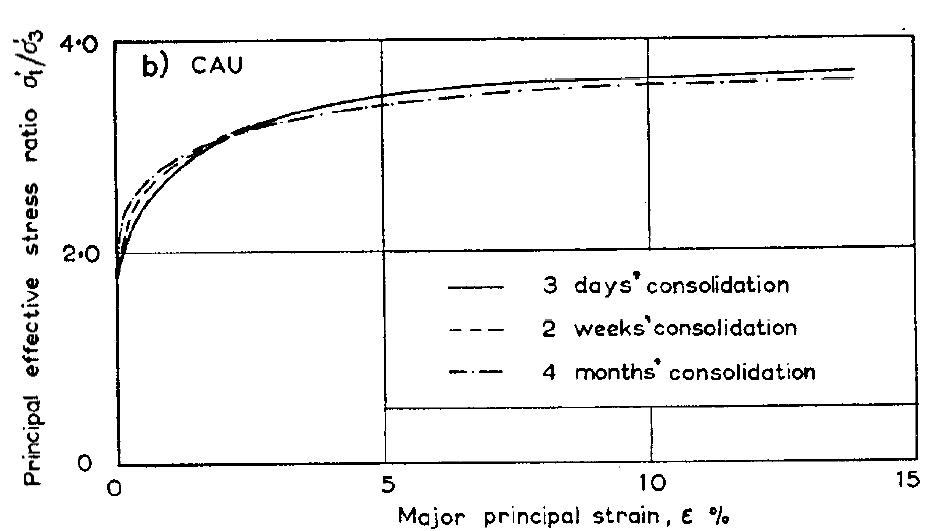
\includegraphics[width=0.48\textwidth]{figures/figure-5a.png}
    }
    \subfigure[CAU, tests on anisotropically consolidated samples]{
        \label{figure:5b}
        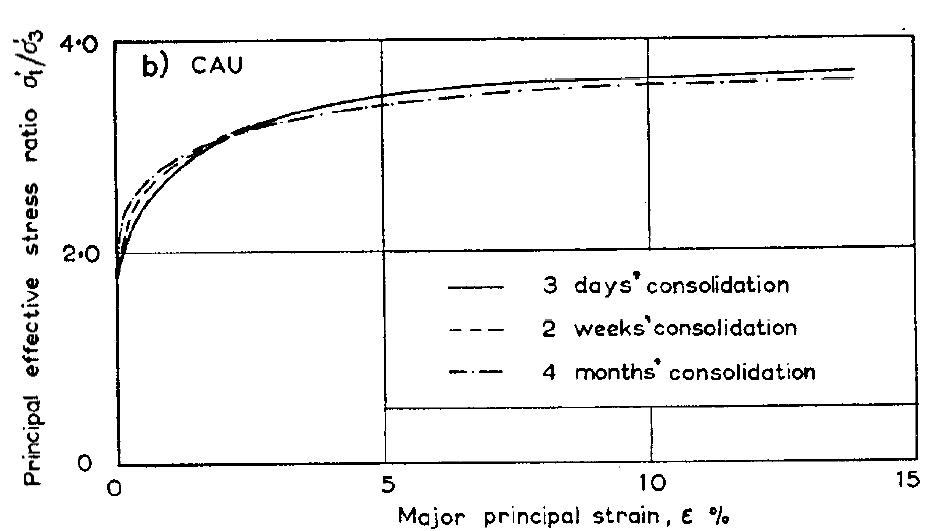
\includegraphics[width=0.48\textwidth]{figures/figure-5b.png}
    }
    \caption{Principal effective stress ratio as observed in consolidated undrained tests, Each curve represents the average of two tests.}
    \addtocounter{figure}{-1}
    \vspace{-5pt}
    \renewcommand{\figurename}{图}
    \caption{固结不排水试验中观察到的主要有效应力比,每条曲线代表两次试验的平均值。}
    \renewcommand{\figurename}{Figure}
    \label{figure:5}
\end{figure}